\chapter{DEVELOPMENT EVALUATION}
\label{app:development}
\label{sec:development-evaluation}
Before participant data collection, the system was evaluated in two ways: automated software verification and recorded development sessions on the headset. Both describe how the apparatus behaves; neither provides participant results or a voice-condition effect.

\section{Software Verification}
Software verification records document the apparatus alongside the development recordings in Section~\ref{sec:development-results}. A verification run on October 20, 2026 passed schedule and voice-isolation checks confirming one practice trial in the first assigned voice, two measured blocks, and the nominal-angle quotas. The same run passed 38 trial-export tests and seven workload scoring and plotting tests, and the Android application was built, installed, and launched successfully. These test counts come from that run and were not re-executed for this manuscript. The current software version, dated October 25, 2026, includes the pre-cue snapshot and balanced direction and height allocation. Its schedule checks pass across 50 participant identifiers and both voice orders, and its geometry checks pass across every starting wall and angle category. These checks predate the change to 32 trials per block and will be repeated on the revised schedule.
\begin{table}[htbp]
\centering\caption{Apparatus verification and outstanding validation.}
\small\tagpdfsetup{table/header-rows={1}}
\begin{tabularx}{\linewidth}{@{}p{0.28\linewidth}XX@{}}\toprule
Component & What was verified & Not yet established \\\midrule
Schedule and voice checks & One practice trial and nominal allocation of 40 trials in each of two blocks pass automated checks & Wearer completion of a full session \\
Trial export and TLX tests & Declared scales and retrospective joins are correct in tested cases & Validation of all questionnaires \\
Unity integration checks & Listed state and interaction cases pass & Robustness to all timing races \\
Android build/install/launch & Application built, installed, and started & Acceptance in a participant session \\
Exact pre-cue theta & Snapshot saved at readiness completion; geometry checks pass & Observation in a complete wearer session \\
Vertical allocation & 20/20 and per-angle height quotas pass schedule checks & Target visibility and seated comfort \\
Voice-condition outcomes & None; no confirmatory dataset reported & Any performance or preference conclusion \\\bottomrule
\end{tabularx}
\end{table}

\section{Recorded Development Results}
\label{sec:development-results}
The descriptive results in this section come from development headset recordings rather than simulated trials. The analysis includes all nine locally mirrored \texttt{DEV\_NEUTRAL} recordings dated October 19--20, 2026 (Runs 20--28), with 27 started searches and 21 recorded correct selections. These sessions used the neutral-male development mode; the eight available trial summaries identify the Eric voice and a 168-object layout. This earlier development configuration differs from the planned participant-study stimuli, and in these sessions guidance decisions were made by the cloud language model Jev rather than by the local decision model described in Section~\ref{sec:decision-model}. Each recording comes from a different software build, and the recordings do not constitute a sample of independent participants. The results therefore describe system operation during development. They estimate neither a self-similar versus neutral voice effect nor differences between software versions.

The analysis retains unfinished searches and uses the complete recorded prefix of Run 21, whose final JSON record is truncated. No missing endpoint is reconstructed. Source file hashes, recording identifiers, derived CSV tables, and the plotting script accompany the thesis sources under \texttt{development-results/}. Twenty of the 21 completed-search durations also match the separately saved trial summaries within their 0.01-second rounding precision; Run 21 has no corresponding summary in the inspected mirror. This comparison checks agreement between exports, not independent timing accuracy.

\subsection{Search Completion During Development}
Figure~\ref{fig:development-search} separates completed-search durations from recording coverage. Panel~(a) shows each completed search, with box plots for runs containing at least three completions; runs with fewer completions show individual observations only. Runs with no recorded completion remain labeled with zero observations. Panel~(b) includes all 27 started searches and identifies the six unfinished searches. Unfinished searches are treated neither as completion times nor as task failures, because a recording may end while the user is testing, pausing, or leaving the application. The logarithmic duration axis retains the longest completed search while allowing shorter searches to remain distinguishable.

The figures use compact, labeled panels and distribution summaries, following the presentation of descriptive results in Chiossi et al.~\cite{chiossi2024searching}. Boxes span the first and third quartiles, the central line marks the median, and whiskers extend to the most extreme observations within 1.5 interquartile ranges. Every observation remains visible as a point, including values beyond the whiskers. Horizontal offsets separate points for legibility without altering measured values, and colors distinguish adjacent runs rather than voice conditions. No confidence intervals or significance annotations are estimated from these recordings.

Among the 21 completed searches, the median recorded active-search duration is 19.56~s, the 95th percentile is 44.43~s, and the maximum is 275.92~s. Percentiles use linear interpolation between ordered observations. The long completed search is retained rather than removed as an outlier. These were unconstrained development sessions, and the logs do not establish that every active second represents uninterrupted task-directed effort. The plotted counter follows the application's search-timer logic, which excludes some intervals, and therefore differs from elapsed recording time. The distribution shows that the application records completed selections and variable search durations. It is not an estimate of participant efficiency under a standardized protocol.

\begin{figure}[htbp]
\centering
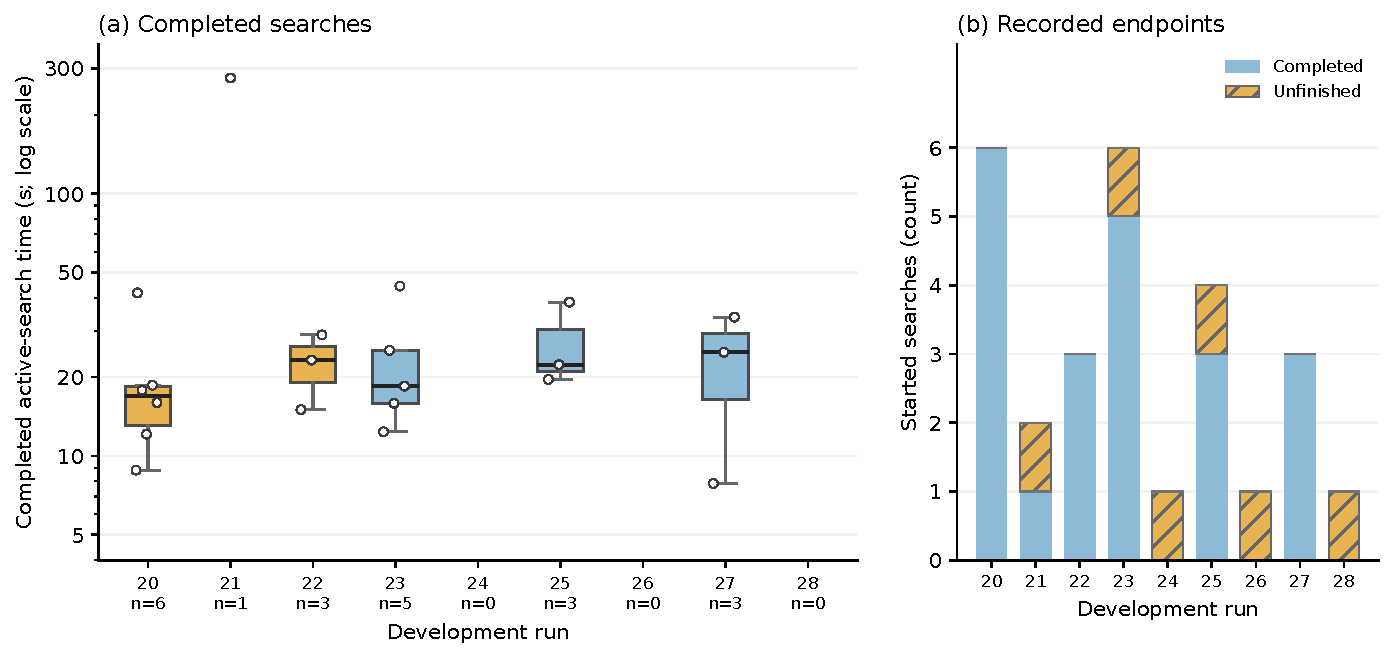
\includegraphics[width=\linewidth,alt={Two panels show development Runs 20 through 28: 21 completed search durations as individual points and quartile boxes on a logarithmic seconds axis, and counts of 21 completed and six unfinished searches. Runs without completions are labeled n equals zero.}]{figures/development-search-times.pdf}
\caption[Recorded development search durations]{Recorded development searches. (a) Completed active-search times, with individual observations, sample counts, and quartile boxes where at least three observations are available; the vertical axis is logarithmic. (b) Counts of completed and unfinished searches. Unfinished searches are excluded from duration summaries, not assigned a completion time.}
\label{fig:development-search}
\end{figure}

\subsection{Speech Delivery and Earlier Waiting}
Of 350 software playback-start events during the recorded search intervals, 339 have an unambiguous chronological match to a guidance request, audio request, and audio-ready event using the same recording, trial, and decision identifier. The remaining 11 playback events are excluded from the latency distribution, rather than assigned zero delay, because the required join is missing or ambiguous. Requests that never produced playback are likewise outside this delivered-event distribution.

For the 339 matched events, the median interval from the delivered decision's request to software playback is 0.244~s, with a 95th percentile of 0.487~s and a maximum of 0.538~s (Figure~\ref{fig:development-speech}). The median request-to-audio-request interval is 215.7~ms, compared with 17.9~ms from audio request to readiness and 1.0~ms from readiness to playback. The first interval can include decision-making and scheduling and so does not isolate Jev network latency. All timestamps mark software events rather than the onset of audible sound at the headset.

\begin{figure}[htbp]
\centering
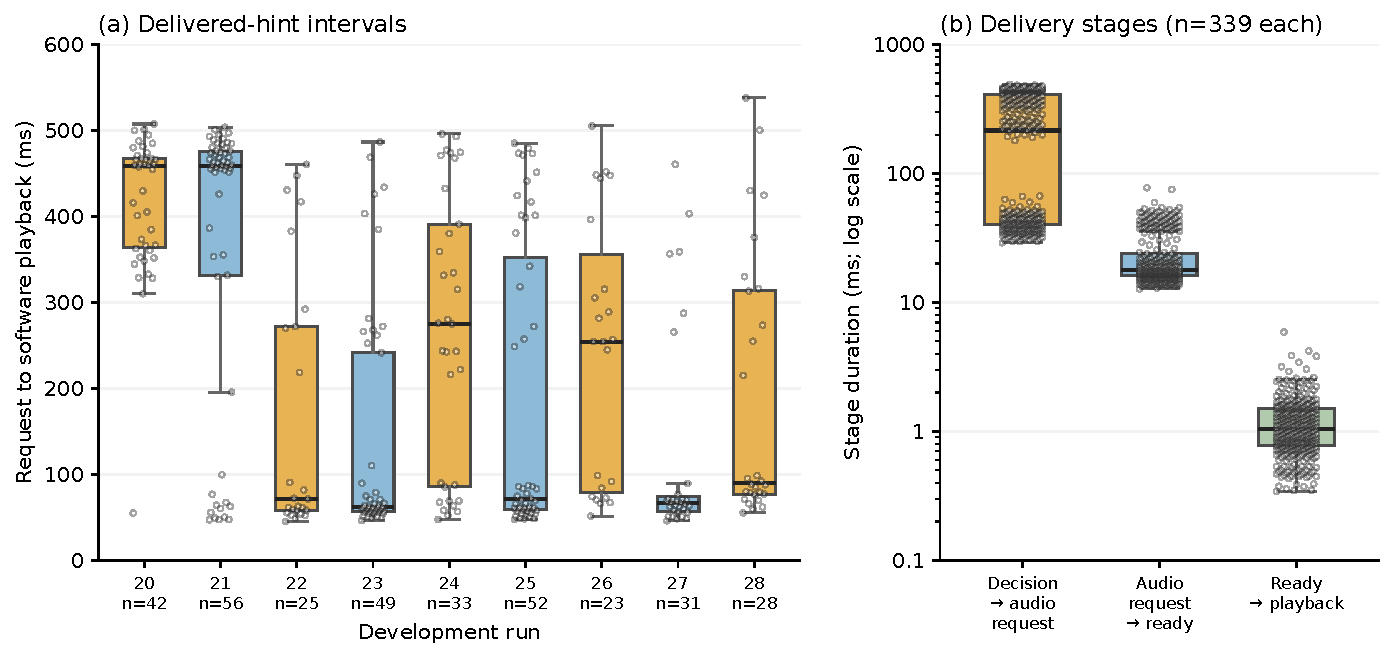
\includegraphics[width=\linewidth,alt={Two panels show 339 matched delivered hints: request-to-playback distributions by development run on a linear milliseconds axis, and the three recorded delivery-stage distributions on a logarithmic milliseconds axis. Each panel shows individual recorded events and quartile boxes.}]{figures/development-speech-delivery.pdf}
\caption[Software speech-delivery intervals]{Software speech-delivery intervals for 339 matched playback events. (a) Request-to-playback distributions by run, with sample counts. (b) Delivery-stage distributions for the same events, using a logarithmic vertical axis. Points retain all observations; boxes and whiskers follow Figure~\ref{fig:development-search}. Earlier qualification and deferral, undelivered requests, and acoustic onset are outside this measure.}
\label{fig:development-speech}
\end{figure}

Short delivery intervals alone do not establish prompt feedback from the user's perspective. Figure~\ref{fig:development-confirmation} reconstructs the gaze-confirmation episode in Run 20, Trial 4. A gaze-qualified hint request is recorded at session time 321.426~s. Three successive transmission snapshots record qualified target gaze, while controller-hold qualification is false. Jev returns \emph{wait}, \emph{wait}, and then \emph{speak}; playback of ``You've got it!'' begins at 323.616~s. The interval from the first qualified request to playback is therefore 2.190~s, although the final request-to-playback interval is only about 0.352~s. The trace is one delayed episode with repeated requests rather than three independent confirmation failures. The snapshots document qualification at those instants but not uninterrupted fixation between them.

\begin{figure}[htbp]
\centering
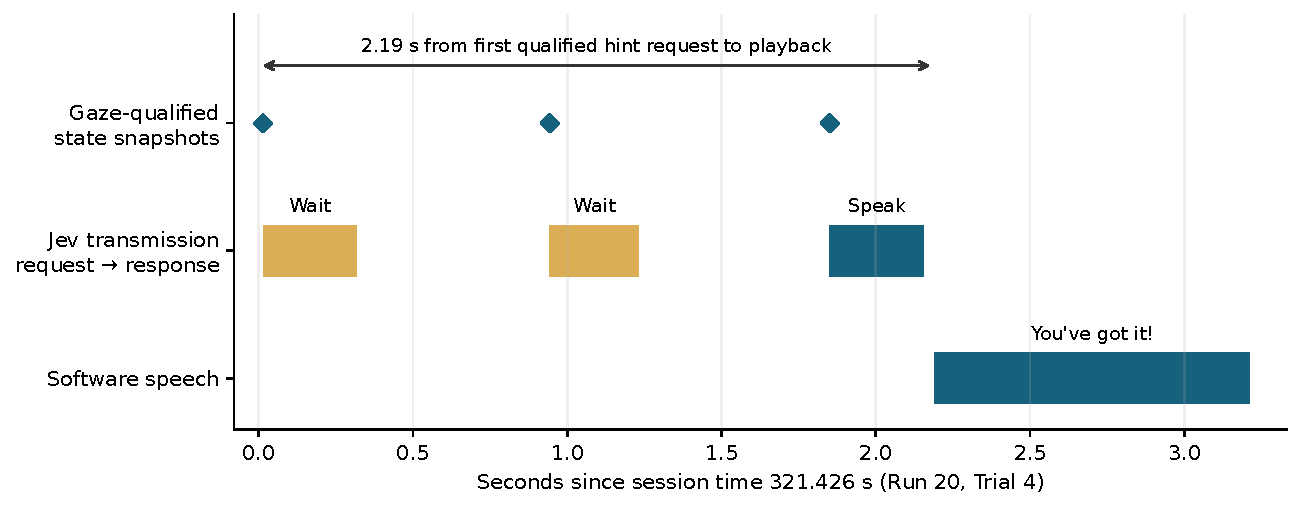
\includegraphics[width=\linewidth,alt={Run 20 Trial 4 timeline: three gaze-qualified snapshots accompany two wait decisions and a speak decision. The confirmation begins 2.19 seconds after the first qualified request. Controller hold is unqualified at all three snapshots.}]{figures/development-confirmation-sequence.pdf}
\caption[Recorded gaze-confirmation delay]{Recorded gaze-confirmation delay in Run 20, Trial 4. Diamonds mark qualified-state snapshots, bars mark transmission request/response intervals and software speech. Gaze confirmation is distinct from controller confirmation and correct trigger selection.}
\label{fig:development-confirmation}
\end{figure}

This case illustrates why sequence histories are needed alongside aggregate delivery statistics. Earlier waiting remains visible even when the request that ultimately produces speech is processed quickly. Whether later software changes eliminated this behavior can be determined only from a comparable recording with the current version. No acoustic-latency or participant-perception conclusion is drawn from this trace.

\subsection{Recorded Gaze Usability}
Figure~\ref{fig:development-gaze} summarizes 58,041 rendered-frame replay samples recorded during active search. A sample is counted as usable when the saved gaze-device availability flag is true and the replay's gaze-usable flag is set. This is the application's recorded usability decision, which includes tracking and freshness checks, rather than a new physiological classification. Samples marked unusable are retained, and absent or indeterminate flags would be classified as unknown.

Across the nine runs, usable-row fractions range from 63.75\% to 99.97\%. All inspected active-search rows have a usable/unusable classification. Intervals with no recorded rows, however, remain unobserved and are not included in the denominator. The dominant logged invalidity reason is \texttt{both\_native\_eyes\_invalid}. This diagnostic alone cannot distinguish among blinking, headset removal, poor fit, calibration, and software issues. Runs with long periods of unusable gaze warrant timeline inspection before they are used to assess guidance behavior.

\begin{figure}[htbp]
\centering
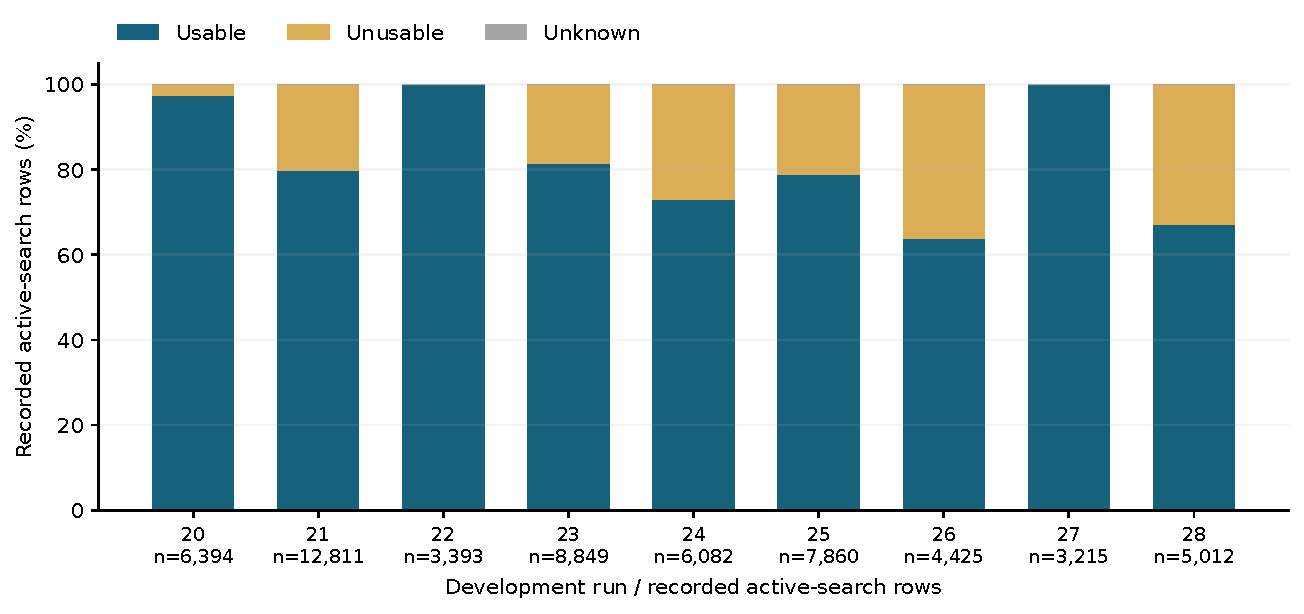
\includegraphics[width=\linewidth,alt={Stacked bars show usable and unusable active-search replay rows for development Runs 20 through 28, with denominators below each bar. Usable fractions range from 63.75 to 99.97 percent; no inspected row has an unknown flag.}]{figures/development-gaze-usability.pdf}
\caption[Recorded gaze usability during development]{Recorded gaze usability during active search, with the number of replay rows shown for each run. These are rendered-frame observations, not independent native sensor samples. Unrecorded intervals are outside the denominator.}
\label{fig:development-gaze}
\end{figure}

The row fractions are diagnostic. They identify differences in the evidence available to the guidance system during these recordings, and they do not estimate spatial accuracy, native acquisition frequency, fixation quality, or the proportion of total search time with valid gaze. Together, the search, delivery, and usability plots characterize the apparatus ahead of the planned voice comparison. They do not address performance or experience differences between voices.

\subsection{Exploratory Eye-Measurement Pipeline}
\label{sec:development-eye-candidates}
A separate analysis uses the recorded eye-observation file for development Run 30 (October 23, 2026), which contains five recorded search identifiers in neutral-male mode. These searches predate the 25-second deadline, and their durations are not truncated. Figure~\ref{fig:development-eye-candidates} presents per-eye candidate fixation counts, candidate saccade rates, exploratory IPA~\cite{duchowski2018ipa}, and pupil duration retained for IPA. The figure uses only measured records; artificial test signals used to verify the code are excluded.

The strict pupil screens retain approximately 2.18, 2.25, 4.22, and 5.28 seconds per eye for the first four searches, with no accepted segment for the fifth. These short retained windows do not represent whole-trial workload, and unavailable IPA values are treated as missing rather than zero. Separate left- and right-eye values expose disagreement rather than averaging it away. The candidate fixation counts and restricted saccade rates likewise depend on detection thresholds and on the available query-time evidence. Three illustrative parameter variants are exported for sensitivity inspection, without choosing a setting on the basis of a favorable result.

\begin{figure}[htbp]
\centering
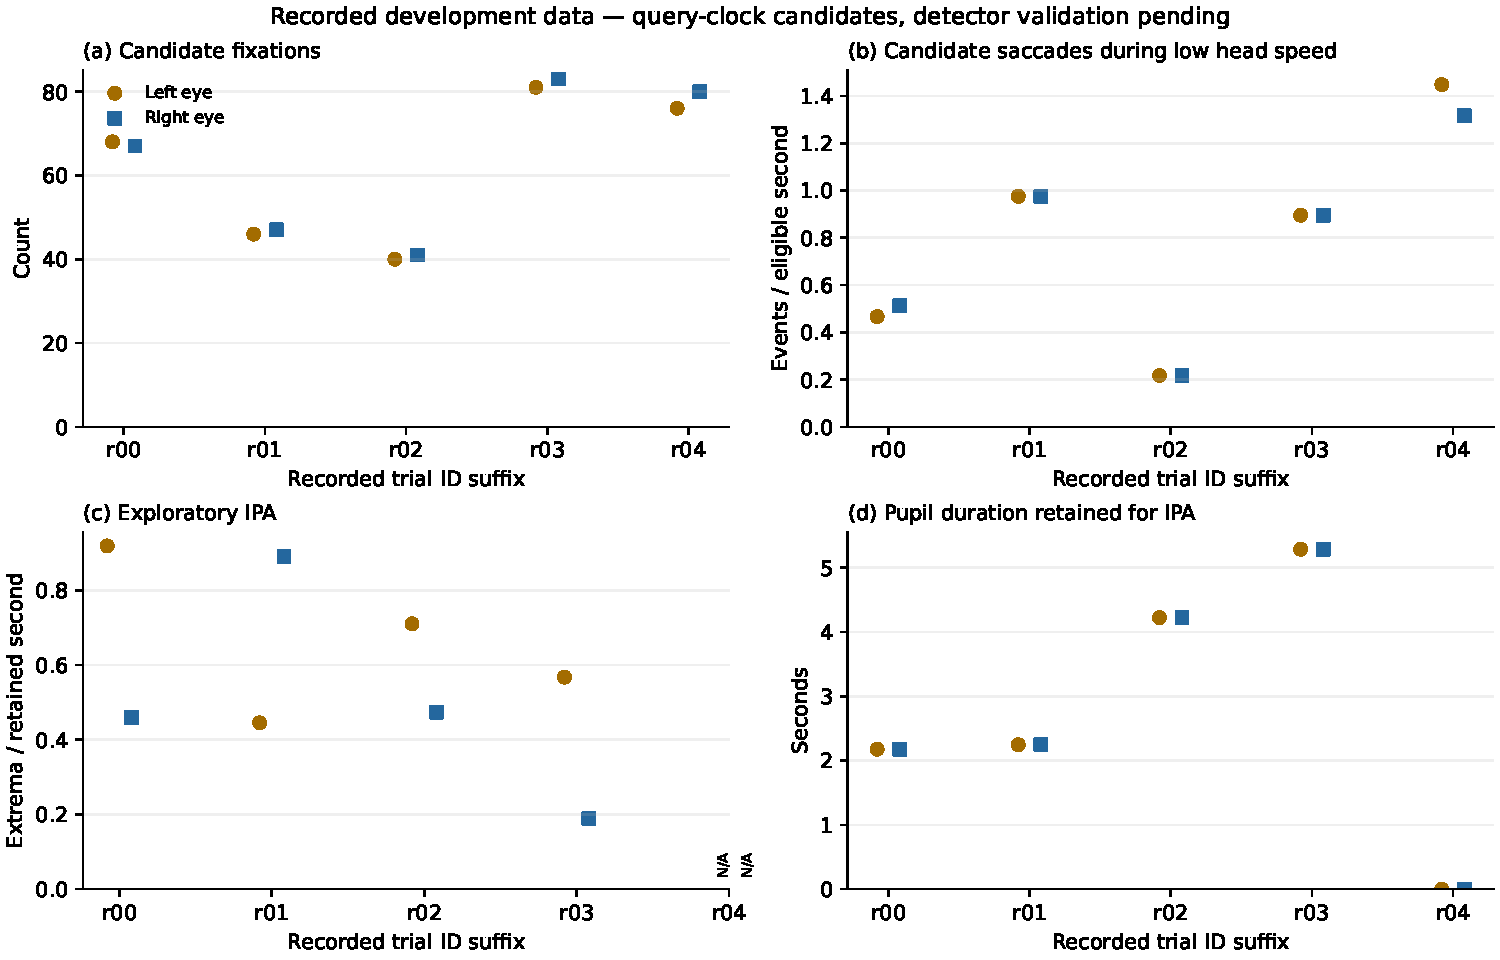
\includegraphics[width=\linewidth,alt={Four panels show actual Run 30 per-eye candidate fixation counts, saccade rates during low head speed, exploratory IPA and retained pupil duration for five searches. The fifth search has unavailable IPA. All eye-event classifications remain unvalidated.}]{figures/development-eye-candidates.pdf}
\caption[Exploratory eye-measurement output from recorded data]{Run 30 development diagnostics. (a) Candidate fixation counts. (b) Candidate saccade events per retained low-head-speed second. (c) Exploratory IPA extrema per retained pupil second. (d) Retained pupil duration. Points represent separate eyes within recorded searches, not independent participants. The software-query clock does not establish 120-Hz sensor acquisition, and the classifications require independent validation.}
\label{fig:development-eye-candidates}
\end{figure}

The source hash, detector configuration, dependency versions, individual event intervals, summary CSV, and threshold-sensitivity table are retained with the thesis development artifacts. The computational checks pass, but without an independently labeled headset sequence, event precision, recall, and duration error cannot yet be established. These results demonstrate an executable measurement workflow and its data limitations rather than participant-study findings.

\subsection{Outcome Panels by Voice Condition}
\label{sec:development-voice-panels}
Figure~\ref{fig:development-voice-panels} adapts the four-panel presentation of accuracy, missed targets, search time, and pupil activity in Chiossi et al.~\cite{chiossi2024searching} to the present study's voice conditions. Each horizontal axis distinguishes \emph{Neutral voice} from \emph{Self-similar voice}; AR/VR and physical/virtual subdivisions are not factors in this comparison. The observations come from development Run 30, whose five started searches all use the neutral voice; the self-similar position therefore contains no observations. Scheduled searches that never started do not contribute observations.

First-selection accuracy is 80\%: four of the five completed searches contain no incorrect trigger selection before the correct selection. This is a run-level proportion among completed searches, rather than a distribution across participants or a measure of success before the 25-second deadline. Active-search completion times use the recorded search counter and retain their original values in seconds. Run 30 has no recorded 25-second deadline, so its missed-target percentage is unavailable; searches lasting longer than 25 seconds are not retrospectively classified as misses.

For the condition-level display, exploratory IPA is the arithmetic mean of the available left- and right-eye candidate rates within each search. Four searches have values from both eyes; the fifth has no eligible pupil segment and remains missing. This display summary is not a validated workload score; the separate-eye diagnostics and retained durations appear in Figure~\ref{fig:development-eye-candidates}. Points in the time and IPA panels are repeated trials within one development run rather than independent participants, and the figure supports no estimate of a voice-condition effect. The participant-study comparison will use observations from both voices and paired participant summaries with consistent scoring and eligibility rules.

\begin{figure}[htbp]
\centering
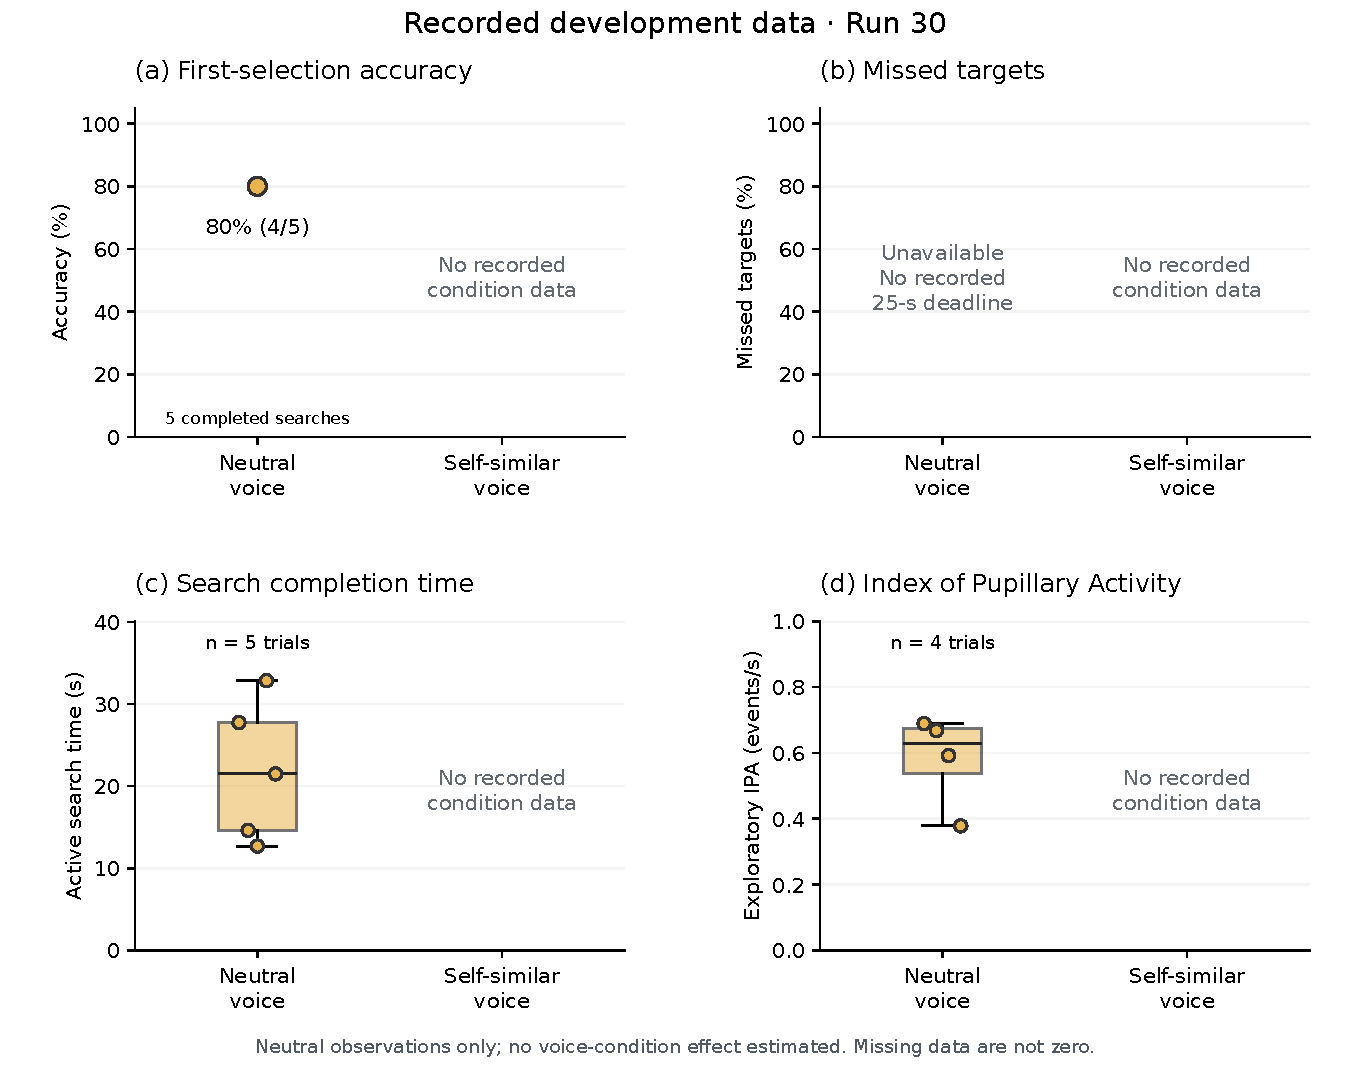
\includegraphics[width=\linewidth,alt={Four development outcome panels use Neutral voice and Self-similar voice on every horizontal axis. Neutral Run 30 has 80 percent first-selection accuracy among five completed searches, five active search times, and four exploratory IPA trial means. Missed-target percentage is unavailable without a recorded deadline. Self-similar data are absent in every panel.}]{figures/development-voice-condition-panels.pdf}
\caption[Development outcome panels by voice condition]{Development outcome panels arranged for the neutral versus self-similar voice comparison. (a) First-selection accuracy among completed searches, shown as one run-level point. (b) Missed targets, unavailable for this recording without a recorded deadline. (c) Active search completion time. (d) Exploratory IPA averaged across available eyes within each trial. Boxes in (c) and (d) show quartiles and median, with 1.5-IQR whiskers; all observed trial values are shown. Unavailable values are not plotted as zero. No self-similar observations or inferential comparisons are included.}
\label{fig:development-voice-panels}
\end{figure}

\subsection{Eye Measures and Workload in Later Development Runs}
\label{sec:development-eye-measures}
Figure~\ref{fig:development-eye-measures} applies the planned eye-measure and workload panels to three later development recordings from October 25, 2026: neutral-voice run 32 and self-similar runs 1 and 2. Unlike Run 30, these recordings include self-similar playback. All three use the angle-controlled schedule in its shortened development mode, the 25-second search limit, right-trigger selection, and the same guidance-policy version, and each session ended before completing a block. The 22 resolved searches comprise 14 neutral searches (12 completed, 2 timed out) and 8 self-similar searches (7 completed, 1 timed out). They are repeated development trials rather than independent participants or paired sessions.

Candidate fixations come from the dispersion-based detector~\cite{salvucci2000fixations} described in Section~\ref{ch:measurement}, applied to each eye within valid, contiguous search intervals; each plotted value is the mean of the two eyes' counts for one search. Candidate saccade frequency divides each eye's candidate saccades by its eligible seconds, which exclude intervals of rapid head movement, and averages the two rates. Both measures rely on the HTC query-receipt clock rather than a verified sensor capture clock, and neither detector has yet been validated against independent annotations. Last target fixation duration is unavailable because it requires a validated join between eye events, the target's area of interest, and the selection time. Raw NASA-TLX~\cite{hart1988nasatlx} is unavailable because these development sessions collected no questionnaire responses. Both panels are kept so that the missing measures remain visible.

Figure~\ref{fig:development-eye-coverage} reports, for each search, the share of active search time eligible for each detector, taking the lower value of the two eyes. Fixation-eligible coverage was at least 94\% in every search except one neutral search at 47\%, and saccade-eligible coverage ranged from 43\% to 93\%. Because fixation counts are totals over eligible time, they scale with search duration and coverage, and the self-similar searches were longer (median 19.7~s versus 13.4~s). Voice, session, search duration, and coverage therefore vary together, and the differences visible in panels (b) and (c) cannot be attributed to voice. No inferential test is applied. None of the three source recordings closed cleanly, and two end in a truncated record that was omitted. These figures show that the measurement pipeline runs end to end on headset recordings with both voices; they do not estimate a voice effect.

\begin{figure}[htbp]
\centering
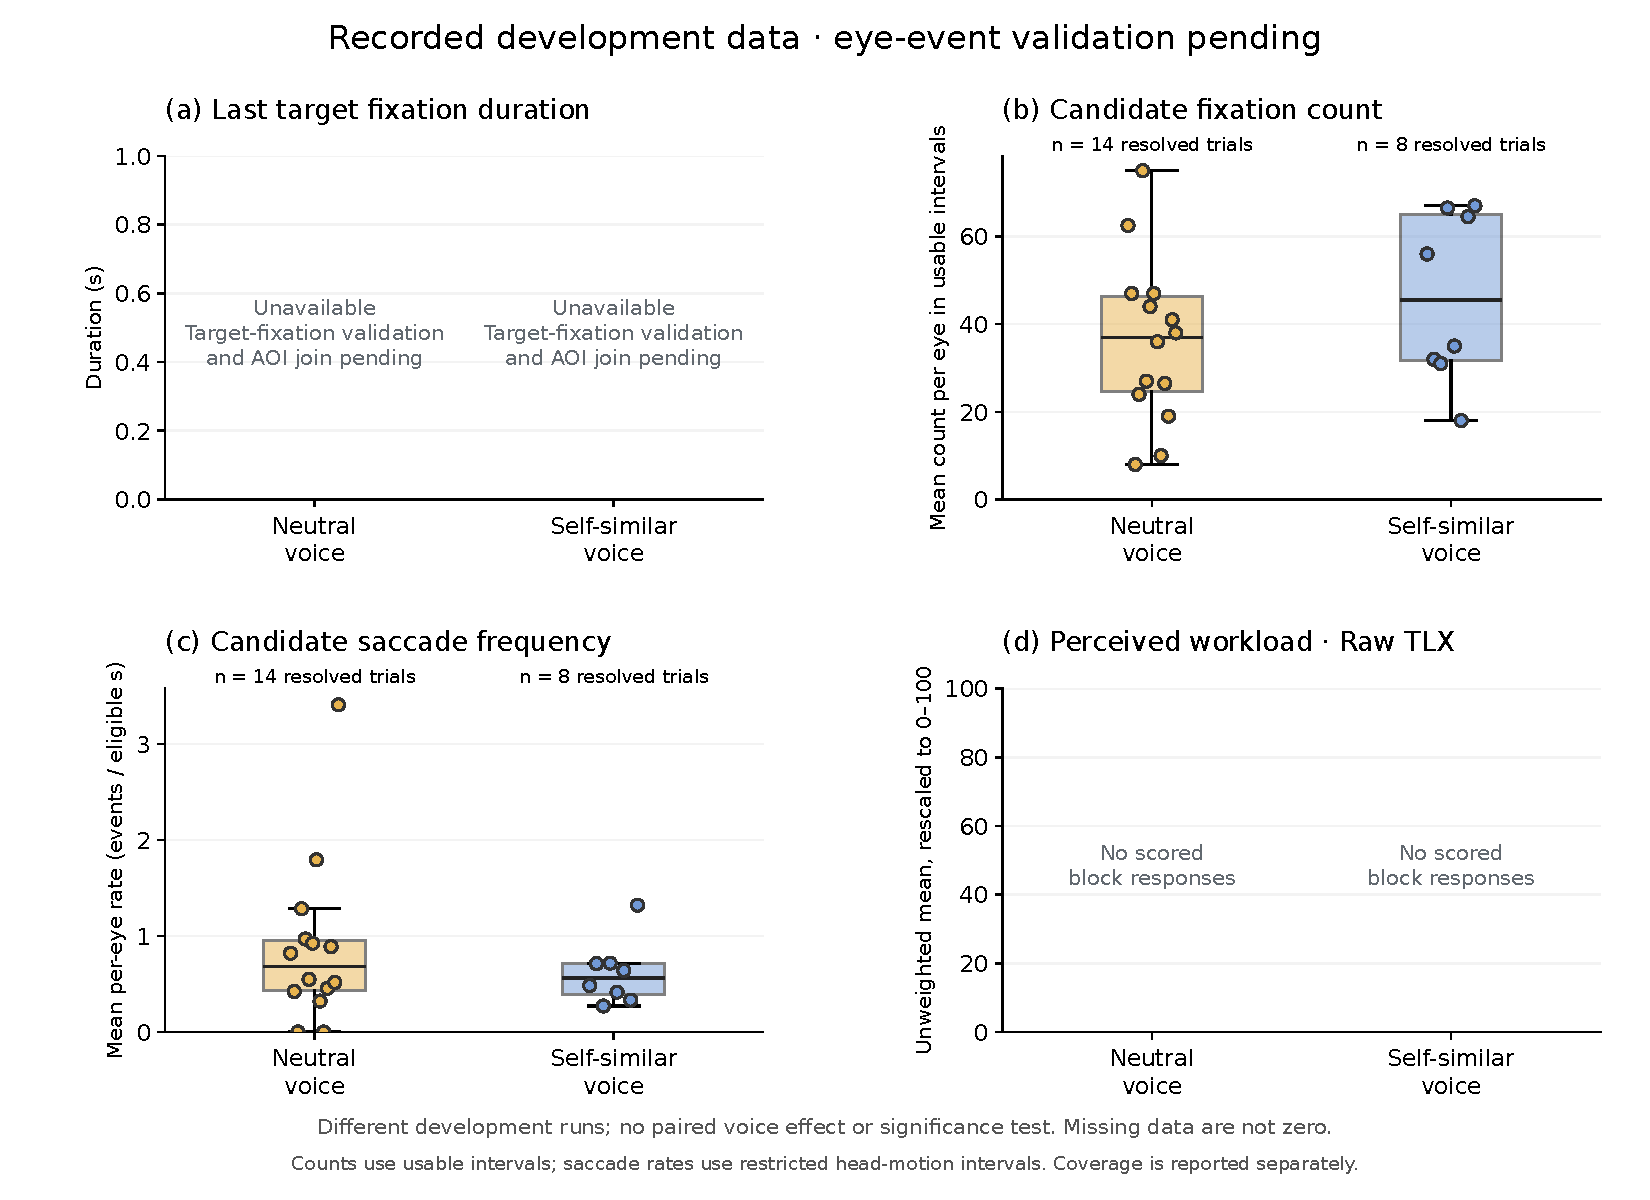
\includegraphics[width=\linewidth,alt={Four panels compare neutral and self-similar development searches. Last target fixation duration and raw NASA-TLX are empty and labeled unavailable. Candidate fixation counts show 14 neutral and 8 self-similar searches; candidate saccade rates show the same searches. Points are individual searches with quartile boxes.}]{figures/development-eye-measures-20261025.pdf}
\caption[Eye-measure and workload panels from development recordings]{Eye-measure and workload panels from October 25 development recordings. (a) Last target fixation duration and (d) raw NASA-TLX are unavailable and are left empty rather than plotted as zero. (b) Candidate fixation count, mean of the two eyes over eligible intervals. (c) Candidate saccade frequency, mean of the two eyes' events per eligible second during low head speed. Each point is one resolved search (neutral run 32, $n=14$; self-similar runs 1 and 2, $n=8$); boxes show quartiles and median with 1.5-IQR whiskers. The detectors are not yet validated, and no inferential comparison is made.}
\label{fig:development-eye-measures}
\end{figure}

\begin{figure}[htbp]
\centering
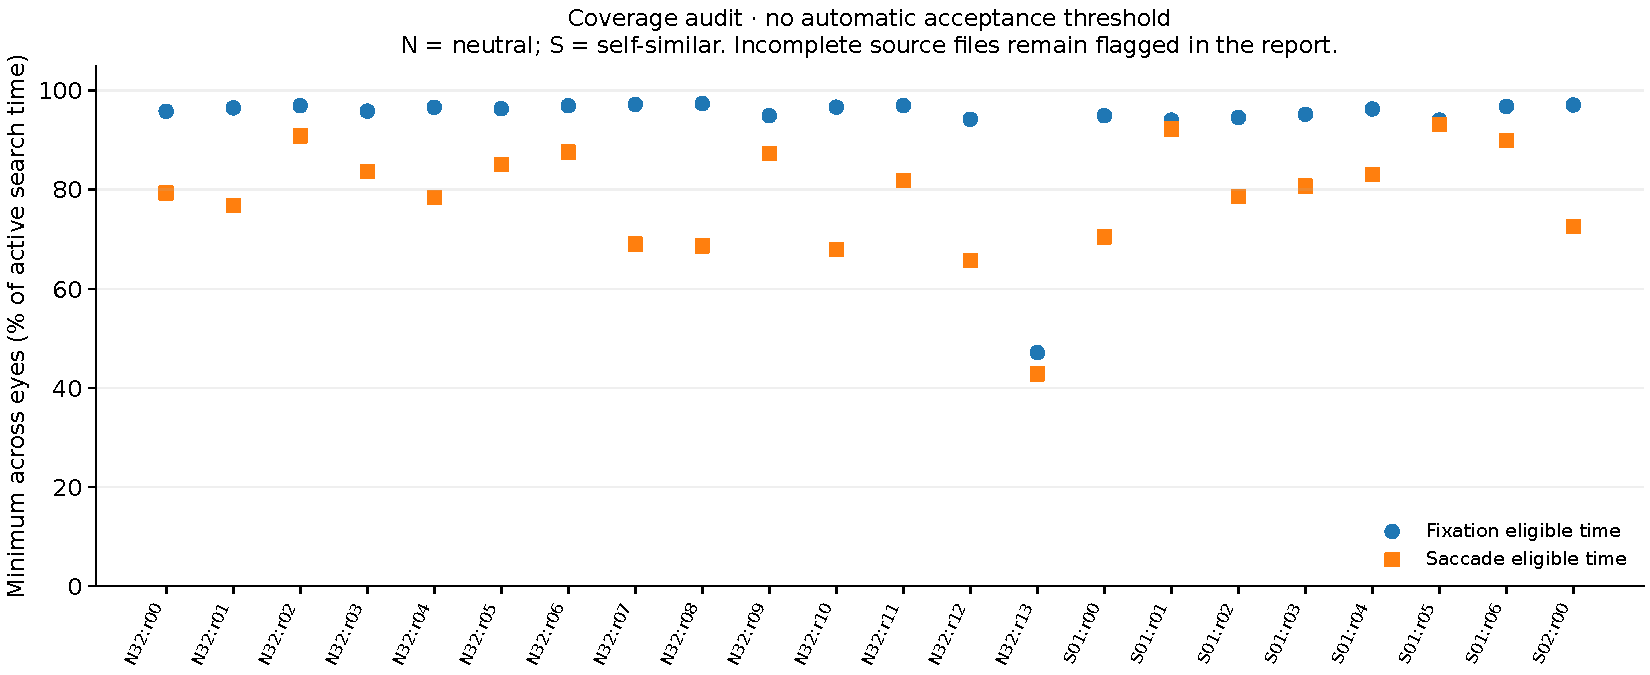
\includegraphics[width=\linewidth,alt={For each of 22 development searches, points show fixation-eligible and saccade-eligible time as a percentage of active search time, using the lower of the two eyes. Fixation-eligible coverage is about 94 to 97 percent except one neutral search at 47 percent; saccade-eligible coverage ranges from about 43 to 93 percent.}]{figures/development-eye-coverage-20261025.pdf}
\caption[Eye-measure coverage in development recordings]{Eye-measure coverage for each search in Figure~\ref{fig:development-eye-measures}, as the percentage of active search time eligible for fixation and saccade detection, using the lower value of the two eyes. N32 denotes neutral run 32; S01 and S02 denote self-similar runs 1 and 2. No acceptance threshold is applied.}
\label{fig:development-eye-coverage}
\end{figure}

\clearpage

